\normalfalse \difficiletrue \tdifficilefalse
\correctiontrue

%\UPSTIidClasse{11} % 11 sup, 12 spé
%\newcommand{\UPSTIidClasse}{11}

\exer{Robovolc $\star$ \label{B2:07:71}}
\setcounter{question}{0}\UPSTIcompetence[2]{B2-07}
\index{Compétence B2-07}
\index{Schéma-blocs}
\index{Robovolc}
\ifcorrection
\else
\marginnote{\textbf{Pas de corrigé pour cet exercice.}}
\fi

\ifprof
\else

On considère le schéma-blocs suivant.
\begin{center}
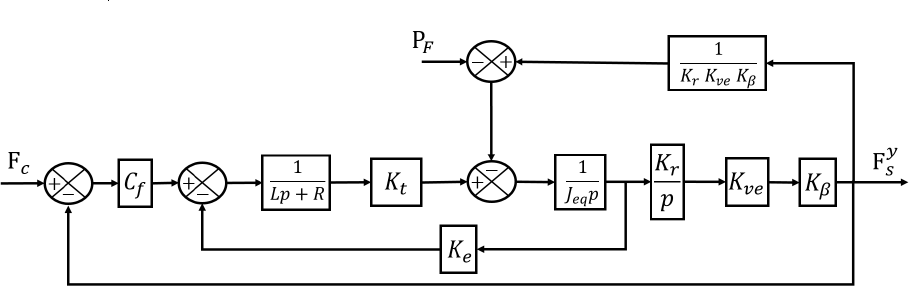
\includegraphics[width=9cm]{71_01}
\end{center}
\fi
\question{En considérant $P_F=0$ (perturbation nulle) et $L=0$ (inductance nulle), calculer la fonction de transfert
$\dfrac{F_S^y}{F_c}$ et la mettre sous la forme canonique $\dfrac{K}{1+Ap+Bp^2}$. Identifier les paramètres $K$,
$A$ et $B$.}
\ifprof
\begin{corrige}

$\dfrac{F_S^y (p)}{F_C (p)}=\dfrac{C_f K_t K_r K_{ve} K_{\beta}}{R+C_f K_t K_r K_{ve} K_{\beta} } \times \dfrac{1}{1+\dfrac{K_e K_t}{R+C_f K_t K_r K_{ve} K_{\beta} }p+\dfrac{RJ_{eq}}{R+C_f K_t K_r K_{ve} K_{\beta} } p^2}$.


Par identification, on obtient :
$K=\dfrac{C_f K_t K_r K_{ve} K_{\beta}}{R+C_f K_t K_r K_{ve} K_{\beta}}$
$A=\dfrac{K_e K_t}{R+C_f K_t K_r K_{ve} K_{\beta} }$;
$B=\dfrac{RJ_{\text{eq}}}{R+C_f K_t K_r K_ve K_{\beta} }$.

\end{corrige}
\else
\fi

 
 \ifprof
\else
\ifcolle
\else
\footnotesize
\noindent
\begin{tabular}{|p{.95\linewidth}|}
\hline
\begin{enumerate}
\item $K=\dfrac{C_f K_t K_r K_{ve} K_{\beta}}{R+C_f K_t K_r K_{ve} K_{\beta}}$,
$A=\dfrac{K_e K_t}{R+C_f K_t K_r K_{ve} K_{\beta} }$,
$B=\dfrac{RJ_{\text{eq}}}{R+C_f K_t K_r K_ve K_{\beta} }$.
\end{enumerate} \\ \hline
\end{tabular}
\normalsize
\fi

\fi


\ifprof
\else
\begin{flushright}
\footnotesize{Corrigé  voir \ref{B2:07:71}.}
\end{flushright}%
\fi